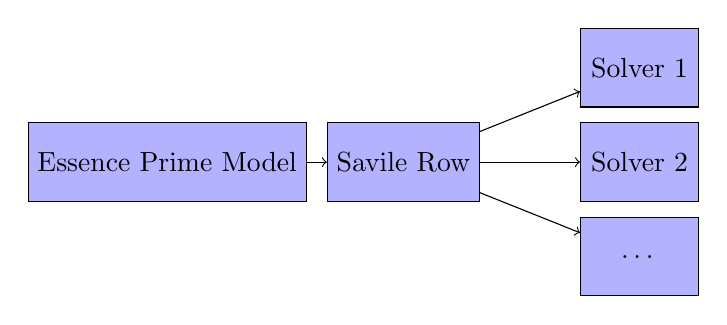
\begin{tikzpicture}[node distance=3cm]
\tikzstyle{file} = [rectangle, minimum width=1.5cm, minimum height=1cm, draw=black, fill=blue!30]
\node (model) [file] {Essence Prime Model};
\node (sr) [file, right of=model] {Savile Row};
\node (sat) [file, right of=sr] {Solver 2};
\node (minion) [file, above of=sat, yshift=-1.8cm] {Solver 1};
\node (other) [file, below of=sat, yshift=1.8cm] {\dots};

\draw[->]             (model) -- (sr);
\draw[->]             (sr) -- (sat);
\draw[->]             (sr) -- (minion);
\draw[->]             (sr) -- (other);
\end{tikzpicture}
